\chapter{Stand der Wissenschaft}
\label{chap:forschungsstand}
Seit den Anfängen der Entwicklung von \gls{open-ran} im Februar 2016 und der Gründung der \orana 2018 gibt es einige wissenschaftliche Arbeiten, die sich mit dem Thema Schwachstellenanalyse und Schwachstellenbewertung in einer \gls{open-ran} Umgebung beschäftigen \autocite{ORANAlliance} \autocite{GuideOpenRAN}. In diesem Kapitel wird ein Überblick über den Forschungsstand anhand einer Auswahl von Arbeiten gegeben.
%
\section{Technischer Report der \orana Security Work Group}
\label{sec:forschungsstand-wg11}
Die \gls{wg11} der \orana beschäftigt sich mit den sicherheitstechnischen Aspekten von \gls{open-ran} und veröffentlicht in regelmäßigen Abständen einen technischen Report, der eine Bedrohungsmodellierung und Risikobeurteilung enthält. Zum Zeitpunkt der Veröffentlichung ist der Report in Version \textit{\textsf{v04.00}} die neueste Fassung dieses Dokuments. Der Report umfasst sowohl mögliche \oran-spezifische Angriffe auf Komponenten und Schnittstellen in einem \gls{open-ran}-System, als auch nicht \oran-spezifische Bedrohungen, wie Supply-Chain-Angriffe auf Quell-Offenen Programmcode oder physischen Eingriff um Zugriff auf sensible Daten zu erlangen, die in allen \glspl{open-ran} existieren können \autocite{o-ranworkgroup11securityworkgroupORANSecurityThreat2024}. Im Folgenden wir ein Überblick über die \oran-spezifischen Bedrohungen gegeben. Die davon betroffenen Komponenten und Schnittstellen sind in Abbildung \ref{fig:oran-architecture} dargestellt.
\begin{figure}
    \centering
    \includegraphics[width=0.5\textwidth]{oran-risk-factors}
    \caption{Einflussfaktoren für die Risikobeurteilung (Quelle: \autocite{o-ranworkgroup11securityworkgroupORANSecurityThreat2024})}
    \label{fig:oran-risk-factors}
\end{figure}
\par Es wird betrachtet wie hoch die Wahrscheinlich (\textit{Likelihood}) ist, dass eine Schwachstelle (\textit{Vulnerability}) durch eine spezifische Bedrohungen (\textit{Threat}) ausgenutzt wird, und welche Konsequenzen (\textit{Consequences}) dies für das Asset hat. Die \orana definiert als Basis für die Risikobewertung eine Reihe von Einflussfaktoren, die in Abbildung \ref{fig:oran-risk-factors} dargestellt sind. Ein Asset ist dabei eine (Teil-)Komponente oder eine Schnittstelle zwischen diesen.  Die \gls{wg11} identifiziert dazu 35 Bedrohungen in der Komponente \textit{O-RAN Cloud} und 69 Bedrohungen die auf alle anderen Komponenten und Schnittstellen zutreffen \autocite[Seite 31 - 69]{o-ranworkgroup11securityworkgroupORANSecurityThreat2024}. Die \orana definiert in ihrem Bericht 102 kritische Assets, also solche, die besonders vor Beeinflussung in den Bereichen Integrität, Verfügbarkeit, Vertraulichkeit, Wiederholbarkeit und Authentizität geschützt werden müssen. Die Verbindung zwischen Bedrohungen und kritischen Assets wird im Bedrohungsinventar hergestellt. Aus der Schweregradbeurteilung und der Eintrittwahrscheinlichkeitsbeurteilung wird der finale Risikowert berechnet. Die Verbindung zwischen einer spezifischen Bedrohung und dem zugehörigen Risikowert stellt das Ergebnis der Risikobewertung dar.
\par Dieser Report gibt keine subjektive Bewertung darüber ab, wie risikobehaftet die Komponenten im System sind. Es handelt sich um eine rein objektive Bewertung, die durch einen Risikowert festgelegt ist. Der Risikowert setzt sich zusammen aus dem Schweregrad und der Wahrscheinlich der Ausnutzung. Der Großteil der Bedrohungen wird dabei in der Risikobewertung mit einem Risikowert von \textit{High} eingestuft, vgl. Abbildung \ref{fig:riskscore-oran-components} \autocite[Seite 130 - 164]{o-ranworkgroup11securityworkgroupORANSecurityThreat2024}.
%
\begin{figure}
    \centering
    \label{fig:riskscore-oran-components}
    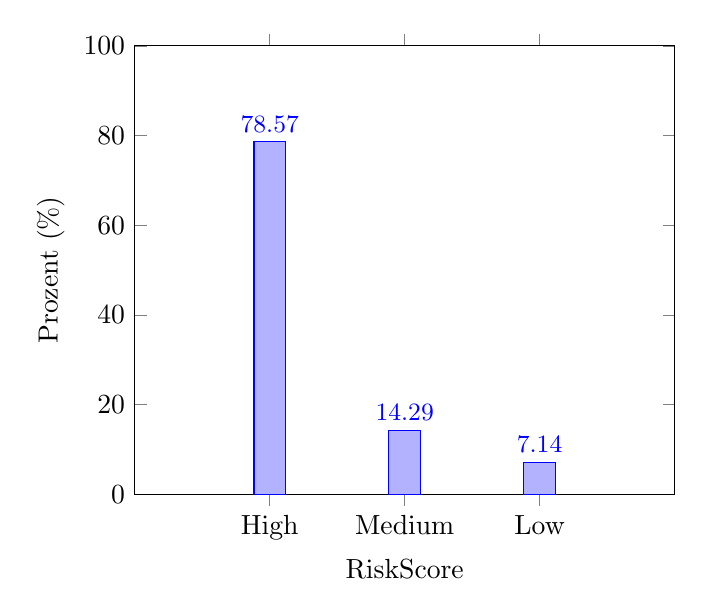
\begin{tikzpicture}
        \begin{axis}[
                ybar,
                symbolic x coords={High, Medium, Low},
                xtick=data,
                ymin=0, ymax=100,
                ylabel={Prozent (\%)},
                xlabel={RiskScore},
                nodes near coords,
                every node near coord/.append style={font=\small},
                bar width=0.4cm,
                enlarge x limits=0.5
            ]
            \addplot coordinates {(High, 78.57) (Medium, 14.29) (Low, 7.14)};
        \end{axis}
    \end{tikzpicture}
    \caption{Risikobewertung der Bedrohungen in \oran Komponenten und Schnittstellen}
\end{figure}
%

\section{BSI Risikoanalyse}
\label{sec:forschungsstand-bsi}
In dieser Studie wird eine weitere Risikoanalyse durchgeführt. Die Studie zielt dabei nicht darauf ab, spezifische Schwachstellen in der Implementierung, sondern in den Spezifikationen der \orana zu finden. \citeauthor{kopsellOpenRANRisikoanalyse2022} führen an, dass die veröffentlichten \oran-Spezifikationen zum Zeitpunkt Februar 2022 nicht viele Vorgaben zur Sicherheit machen und sich insbesondere nicht an dem Ansatz \textit{security/privacy by design/default} orientiert. Als Folge dessen werden viele potenzielle Sicherheitsrisiken mit mittlerem bis hohem Schweregrad festgestellt. Die Studie präsentiert außerdem Maßnahmen, deren Umsetzung zur Verbesserung der Sicherheit in der \oran-Umgebung führen würde \autocite{kopsellOpenRANRisikoanalyse2022}.
\par Weitere umfangreiche Risikoanalysen für 5G oder 5G RAN wurden von \gls{nis} und \gls{enisa} veröffentlicht, diese sind aber nicht auf \gls{open-ran} fokussiert \autocite{europeanunionagencyfornetworkandinformationsecurity.ENISAThreatLandscape2019} \autocite{EUCoordinatedRisk2019}.
%
\section{Empirische Analyse von Schwachstellen im Open RAN Umfeld}
\label{sec:forschungsstand-acema}
\citeauthor{klementSecuring6GTransition2024} untersuchen in ihrem Artikel \textit{\gls{acema-full}} die Sicherheitsherausforderungen, die mit dem Übergang von 5G zu 6G-Netzen und der Einführung von \gls{open-ran}-Technologien einhergehen. Ziel ihrer Forschung ist die Entwicklung eines umfassenden Ansatzes zur Bewertung und Priorisierung von Sicherheitsbedrohungen in \gls{open-ran}-Umgebungen, wobei die O-Cloud-Komponente als repräsentatives Beispiel dient. Hierzu kombinieren die Autoren das \gls{mitre} \gls{attack} Framework mit empirischen Daten, um Bedrohungen in einer O-RAN-Implementierung zu analysieren. Im Zentrum ihrer Methodik steht die Abbildung einer \gls{mitre}-Technik zu einem spezifischen \gls{cve}-Datum über das Durchsuchen der unterschiedlichen Kategorisierungssysteme \gls{capec}, \gls{cwe} und \gls{cve}. Dazu muss in einem manuellen Schritt eine Zuordnung zwischen \oran \textit{Threat-ID} und \gls{mitre}-Technik geschaffen werden. Dieser Schritt ist ohne Probleme durchführbar, da sowohl \textit{Threat-ID} und \gls{mitre}-Technik eine gute Dokumentation aufweisen und über die jeweiligen Beschreibungen eine Verknüpfung gefunden werden kann. Die Anwendung des \gls{cvss}, um den Schweregrad möglicher Schwachstellen zu bewerten, geht über die bisher vorgenommenen Bewertungssysteme der \orana heraus und ermöglicht eine granuläre Auswertung der Ergebnisse. Die Erkenntnisse dieser Arbeit tragen dazu bei, die Sicherheitslücken in \oran zu minimieren, indem Bewusstsein für spezifische Bedrohungsszenarien geschaffen wird. Dies wird durch einfach verständliche Datenvisualisierungen unterstützt. Die Modularität des Ansatzes erlaubt außerdem eine Übertragung auf andere Komponenten neben \textit{O-Cloud} im \oran Umfeld \autocite{klementSecuring6GTransition2024}.

%
\section{Empirische Analyse von Schwachstellen im Android Umfeld}
\label{sec:forschungsstand-android}
Auch in anderen Feldern der Informatik werden empirische Methoden genutzt, um die Sicherheit von Komponenten im jeweiligen System zu analysieren und bewerten.
\par Mit \citetitle{mazuera-rozoAndroidOSStack2019} wurde 2019 eine empirische Studie durchgeführt die, ähnlich wie \gls{acema} im Umfeld von \gls{open-ran}, eine umfangreiche Schwachstellenanalyse und Schwachstellenbewertung auf allen öffentlich auffindbaren Schwachstellen im Android-Umfeld betrachtet. \citeauthor{mazuera-rozoAndroidOSStack2019} betrachten in dieser Studie besonders die Art der Schwachstellen und wie sich diese über den Verlauf der Zeit ändern. Außerdem werden die Angriffsvektoren nach \gls{cvss} analysiert, die angegriffenen Ebenen und Teilsysteme von Android betrachtet und die Frage beantwortet wie lange es dauert, bis die Schwachstellen geschlossen werden. Die Studie nutzt die \gls{mitre} \gls{cwe} Kategorisierung um die spezifischen Schwachstellen\footnote{\textit{Englische Übersetzung}: vulnerabilities} einer übergeordneten Schwachstelle\footnote{\textit{Englische Übersetzung}: weakness} zuzuordnen. Sie kommen zu dem Schluss, dass mindestens 60\% der 1235 betrachteten Schwachstellen eine hohe Auswirkung auf die Vertraulichkeit(60\%), Integrität(60\%) und Verfügbarkeit(65\%) des Geräts haben \autocite[Abbildung 8]{mazuera-rozoAndroidOSStack2019}. Auch wenn die Ergebnisse nicht direkt vergleichbar sind, verdeutlichen \autocite{mazuera-rozoAndroidOSStack2019} und \autocite{klementSecuring6GTransition2024} die Relevanz einer empirischen Analyse und Kategorisierung von Schwachstellen in unterschiedlichen technologischen Kontexten.